\section{三重积分、曲线曲面积分}
	\subsection{三重积分}

	\begin{ti}
		设 $\varOmega_{1} = \bigl\{ (x,y,z) \bigl| 0 \leq x \leq 1, 0 \leq y \leq 1, 0 \leq z \leq 1 \bigr\}$,$\varOmega_{2} = \bigl\{ (x,y,z) \bigl| 0 \leq x \leq 1, 0 \leq y \leq 1, -1 \leq z \leq 0 \bigr\}$,且 $I_{1} = \iiint_{\varOmega_{1}} x y z^{2} \ee^{xyz} \dd{v}$,$I_{2} = \iiint_{\varOmega_{2}} x y z^{2} \ee^{xyz} \dd{v}$,则\kuo.

		\twoch{$I_{1} = I_{2}$}{$I_{1} < I_{2}$}{$I_{1} > I_{2}$}{以上结论都不对}
	\end{ti}

	\begin{ti}
		设 $\varOmega = \Bigl\{ (x,y,z) \Bigl| \frac{x^{2}}{a^{2}} + \frac{y^{2}}{b^{2}} + \frac{z^{2}}{c^{2}} \leq 1, z \geq 0 \Bigr\}$,其中常数 $a > b > c > 0$. 求三重积分 $\iiint_{\varOmega} z^{2} \dd{v}$.
	\end{ti}

	\begin{ti}
		计算 $I = \iiint_{\varOmega} \bigl( x^{2} + y^{2} \bigr) \dd{v}$,其中 $\varOmega$ 为平面曲线 $\begin{cases}
			y^{2} = 2z,\\
			x = 0
		\end{cases}$ 绕 $z$ 轴旋转一周形成的曲面与平面 $z = 8$ 所围成的区域.
	\end{ti}

	\begin{ti}
		计算三重积分 $\iiint_{\varOmega} \bigl| x^{2} + y^{2} + z^{2} - 1 \bigr| \dd{v}$,其中 $\varOmega = \bigl\{ (x,y,z) \bigl| x^{2} + y^{2} + z^{2} \leq 2 \bigr\}$.
	\end{ti}

	\begin{ti}
		设 $\varOmega = \bigl\{ (x,y,z) \bigl| z \leq \sqrt{x^{2} + y^{2}} \leq \sqrt{3}z, 0 \leq z \leq 4 \bigr\}$,计算三重积分 $\iiint_{\varOmega} z \dd{v}$.
	\end{ti}

	\begin{ti}
		设空间区域 $\varOmega = \Bigl\{ (x,y,z) \Bigl| z \geq x^{2} + y^{2}, \frac{\sqrt{\uppi}}{2} \leq z \leq \sqrt{\uppi} \Bigr\}$,则 $\iiint_{\varOmega} \sin z^{2} \dd{v} = $\htwo.
	\end{ti}

	\begin{ti}
		计算三重积分
		\[
			\iiint_{\varOmega} \Bigl( x \sqrt{1 - z^{2}} + y \sqrt{1 - x^{2}} + z \sqrt{1 - y^{2}} \Bigr) \dd{v},
		\]
		其中 $\varOmega$ 由平面 $y = 1$,圆柱面 $x^{2} + z^{2} = 1$ 和半球面 $y = -\sqrt{1 - x^{2} - z^{2}}$ 围成,如图~\ref{fig:1.7.1} 所示.
		\begin{figure}[htbp]
			\centering
			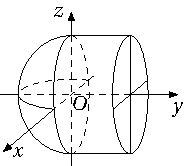
\includegraphics[scale=1]{figure/fig1-7-1.pdf}
			\caption{}\label{fig:1.7.1}
		\end{figure}
	\end{ti}

	\begin{ti}
		求曲面 $z = 2 \bigl( x^{2} + y^{2} \bigr), x^{2} + y^{2} = x, x^{2} + y^{2} = 2x$ 和 $z = 0$ 所围几何体的体积.
	\end{ti}

	\begin{ti}
		设 $f(x)$ 在 $[0,1]$ 上连续,试证:
		\[
			\int_{0}^{1} \dd{x} \int_{0}^{x} \dd{y} \int_{0}^{y} f(x) f(y) f(z) \dd{z} = \frac{1}{3!} \Biggl[ \int_{0}^{1} f(t) \dd{t} \Biggr]^{3}.
		\]
	\end{ti}

	\begin{ti}
		设球体 $x^{2} + y^{2} + z^{2} \leq 2az$(如图~\ref{fig:1.7.2})中任一点的密度与该点到坐标原点的距离成正比,求此球体的重心.
		\begin{figure}[htbp]
			\centering
			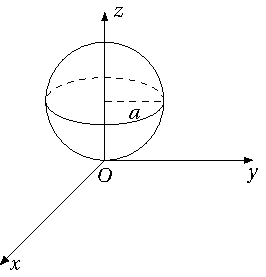
\includegraphics[scale=1]{figure/fig1-7-2.pdf}
			\caption{}\label{fig:1.7.2}
		\end{figure}
	\end{ti}

	\begin{ti}
		在密度为 $1$ 的半球体 $0 \leq z \leq \sqrt{R^{2} - x^{2} - y^{2}}$ 的底面接上一个相同材料的柱体:$-h \leq z < 0, x^{2} + y^{2} \leq R^{2} (h > 0)$,试确定 $h$ 值,使整个球柱体的重心恰好落在球心上.
	\end{ti}

	\begin{ti}
		设 $f(x)$ 为定义在 $[0,+\infty)$ 上的连续函数,且满足
		\[
			f(t) = \iiint_{\varOmega: x^{2} + y^{2} + z^{2} \leq t^{2}} f \Bigl( \sqrt{x^{2} + y^{2} + z^{2}} \Bigr) \dd{v} + t^{3},
		\]
		求 $f(1)$.
	\end{ti}